\section{Vulnerability Scan}

In dieser Aufgabe ging es darum, sich einen Überblick über das Netzwerk zu verschaffen und die potenziellen Ziele voneinander zu unterscheiden bzw. diese anhand ausreichender Informationen den jeweiligen Aufgaben zuzuordnen.\\
Im ersten Schritt wurde mit einem einfachen \texttt{nmap -sP} überprüft, welche Geräte im Netzwerk erreichbar sind, wie in der folgenden Abbildung zu sehen ist:
\begin{figure}[H]
	\centering
	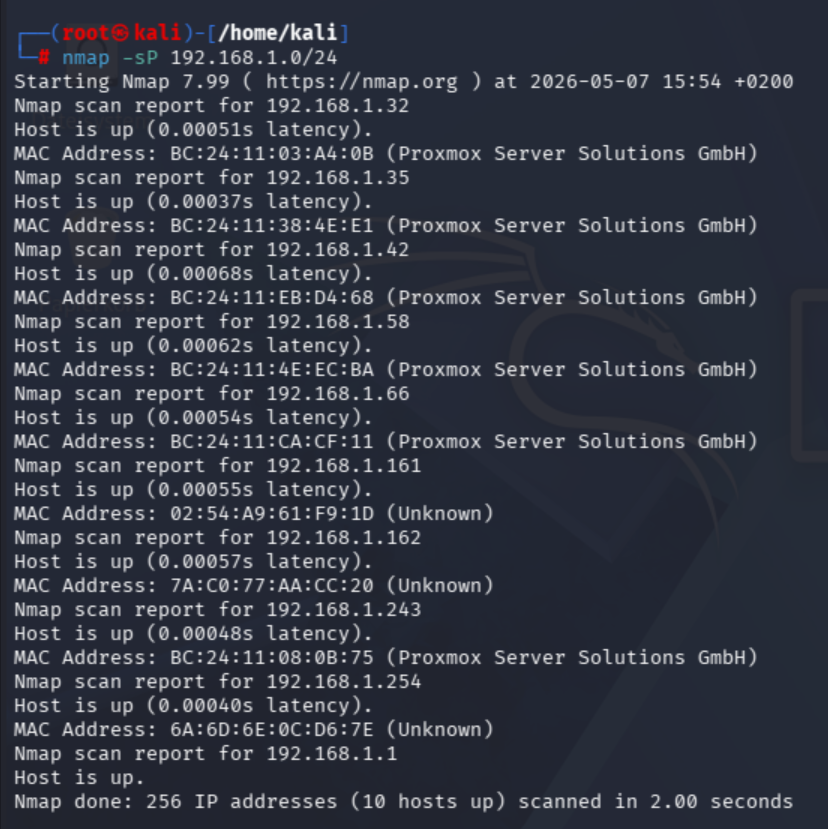
\includegraphics[width=0.85\linewidth]{Whakaahua/aufgabe1/Nmapscan_Aufgabe1_einfacherPing}
	\caption{Nmap Ping}
	\label{fig:nmapping}
\end{figure}
Dabei konnten neben unserem eigenen System insgesamt neun weitere Geräte identifiziert werden. Um detailliertere Informationen zu den einzelnen Hosts zu erhalten, wurde anschließend ein Scan mit \texttt{nmap -sV} durchgeführt. Dieser liefert Informationen über offene Ports sowie die auf den Zielsystemen laufenden Dienste und deren Versionen.
\begin{figure}[H]
	\centering
	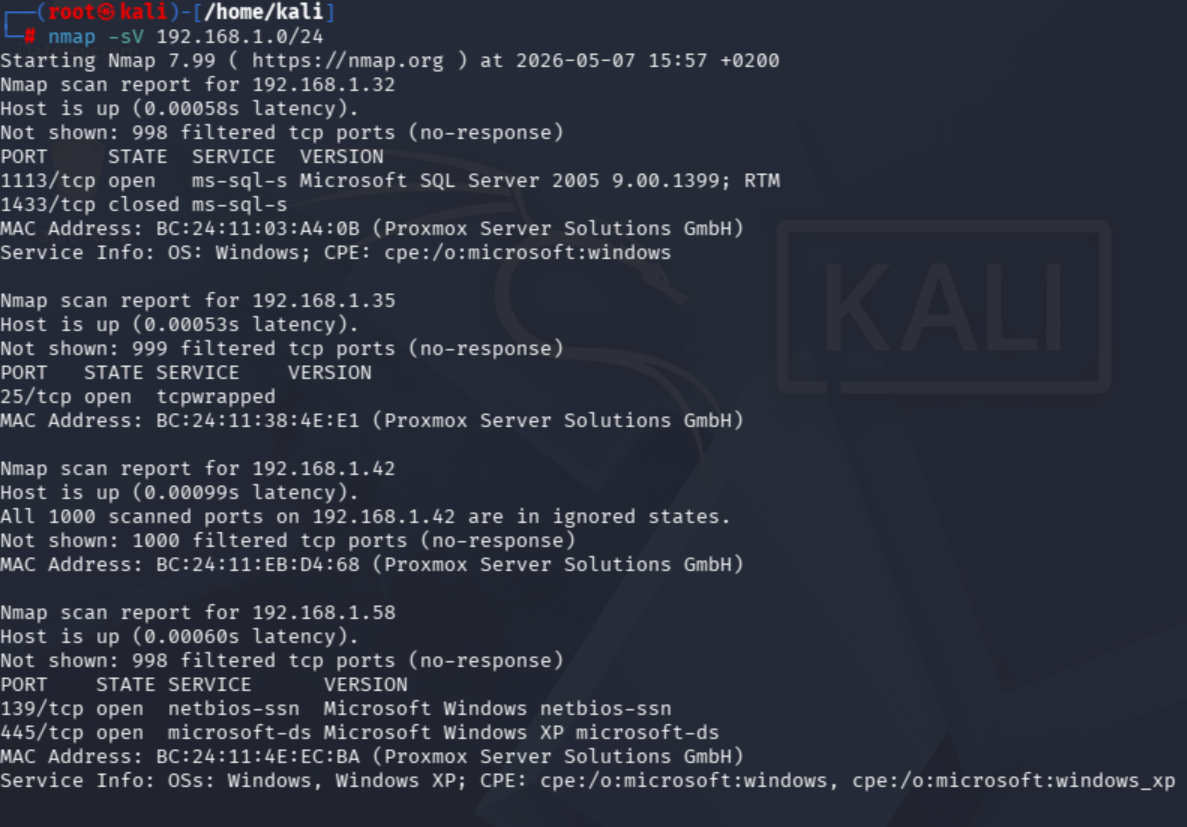
\includegraphics[width=0.85\linewidth]{Whakaahua/aufgabe1/nmap_sv_35_42_58}
	\caption{Nmap Scan}
	\label{fig:nmap35}
\end{figure}

\begin{figure}[H]
	\centering
	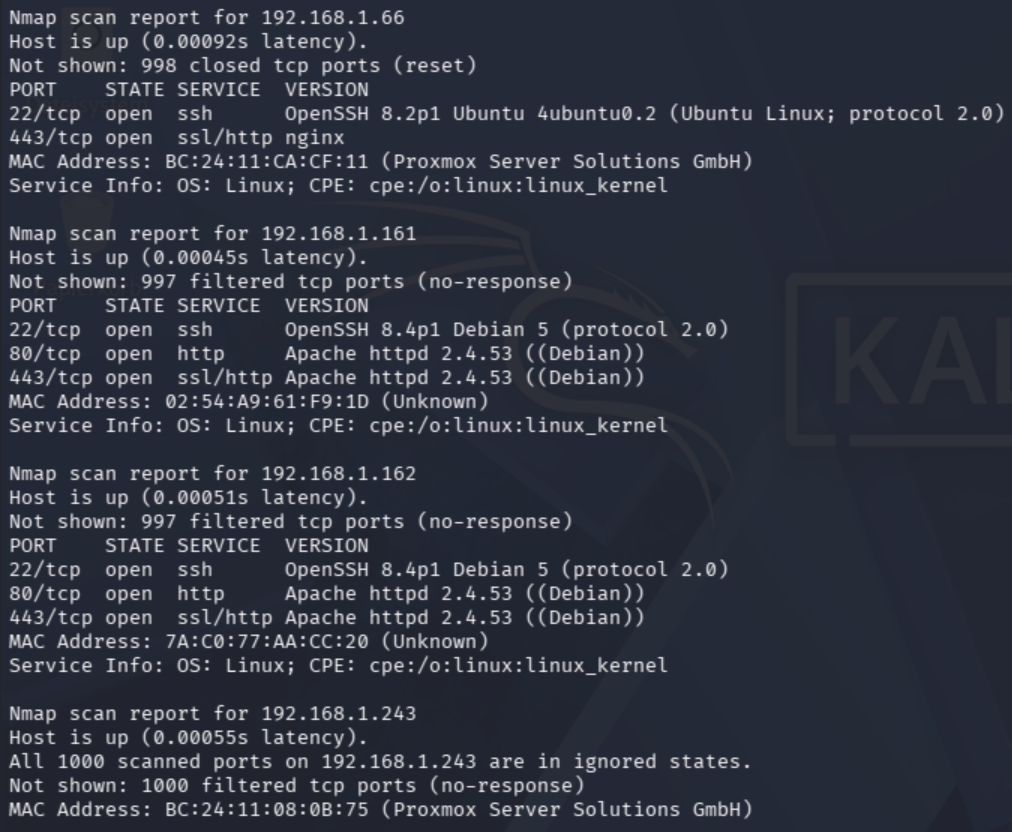
\includegraphics[width=0.85\linewidth]{Whakaahua/aufgabe1/nmap_sv_66_161_162_243}
	\caption{Nmap Scan}
	\label{fig:nmap}
\end{figure}

\begin{figure}[H]
	\centering
	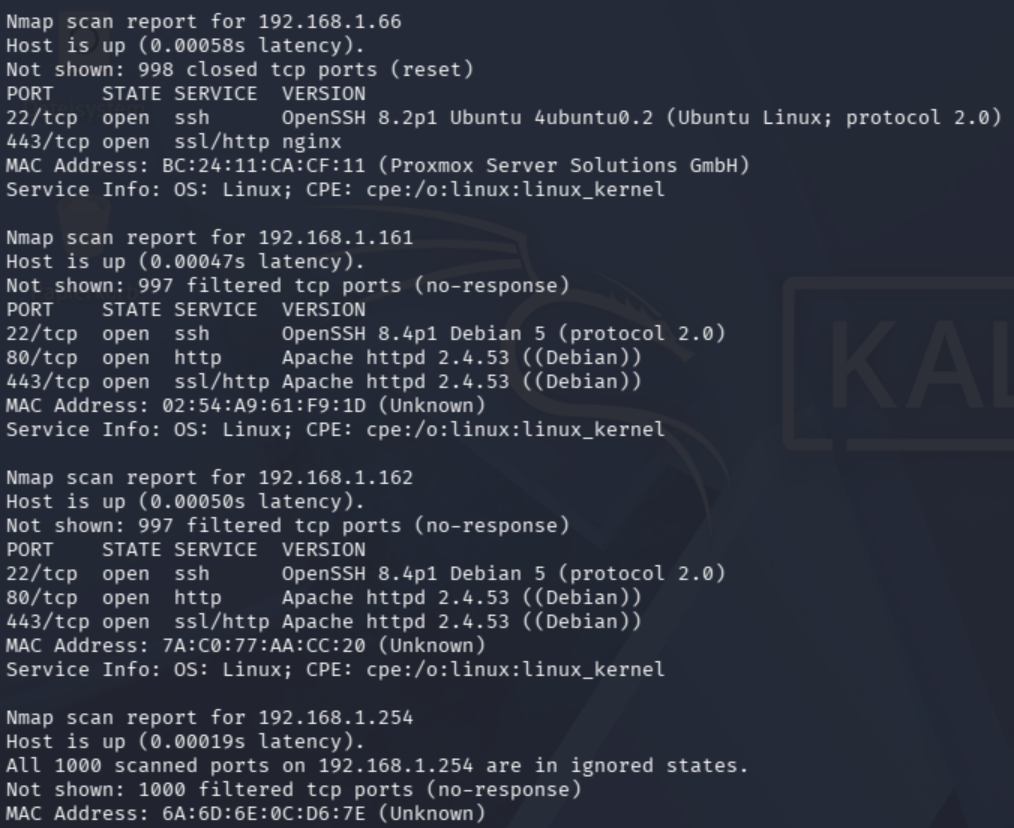
\includegraphics[width=0.85\linewidth]{Whakaahua/aufgabe1/nmap_sv_zusätzlich254}
	\caption{Nmap Scan}
	\label{fig:nmap254}
\end{figure}
Die Ergebnisse zeigen verschiedene Systeme mit unterschiedlichen Diensten und Konfigurationen. Besonders interessant sind dabei veraltete Softwareversionen, da diese häufig bekannte Sicherheitslücken aufweisen. Darüber hinaus konnten mehrere offene Ports identifiziert werden, die potenzielle Einstiegspunkte für weitere Analysen und Untersuchungen darstellen.